\documentclass[]{article}

\author{Braden Fineberg}
\usepackage[pdftex]{graphicx}
\usepackage{achicago}
\usepackage{fullpage}
\usepackage{ amssymb }
\usepackage{amsmath} 
%\usepackage[top=1in, bottom=1in, left= 1 in, right=1in]{geometry}
\usepackage{setspace}
\usepackage[nopar]{lipsum} % for dummy text
\newcommand{\HRule}{\rule{\linewidth}{0.25mm}}

\usepackage{listings}
\usepackage{subfig}
\usepackage{color} %red, green, blue, yellow, cyan, magenta, black, white
\definecolor{mygreen}{RGB}{28,172,0} % color values Red, Green, Blue
\definecolor{mylilas}{RGB}{170,55,241}
\renewcommand\thesection{\Alph{section}}


\begin{document}
	
	\lstset{language=Matlab,%
		%basicstyle=\color{red},
		breaklines=true,%
		morekeywords={matlab2tikz},
		keywordstyle=\color{blue},%
		morekeywords=[2]{1}, keywordstyle=[2]{\color{black}},
		identifierstyle=\color{black},%
		stringstyle=\color{mylilas},
		commentstyle=\color{mygreen},%
		showstringspaces=false,%without this there will be a symbol in the places where there is a space
		numbers=left,%
		numberstyle={\tiny \color{black}},% size of the numbers
		numbersep=9pt, % this defines how far the numbers are from the text
		emph=[1]{for,end,break},emphstyle=[1]\color{red}, %some words to emphasise
		%emph=[2]{word1,word2}, emphstyle=[2]{style},  
		basicstyle=\tiny,  
	}

\input{../title.tex} 

\section{Derivation of (3) and (4)}

Given the fact that the price of a stock can be viewed as a random walk, a form of Brownian Motion, we know that there is some likelihood that tomorrows close price will move up or down in a roughly normal distribution. This concept, combined with the Markovian nature of stock movements allows us to assume that the price is Brownian. Now given the fact that the price is Brownian, with mean $\mu h$ and variance $\sigma^2 h$, we know that the expected change in the stocks price tomorrow is $\mu h$. The equations of (3) and (4) compute the unbiased mean and variance of the Brownian motion over time by looking at independent (due to Markovian stock prices) days of stock change. They capitalize on the central limit theory to compute an expected mean and variance normalized by the number of samples and a scalar h.

\section{Determination of drift and volatility}
Drift and volatility are the difference of two logs. Using the following code, I calculated mu and sigma.

\begin{lstlisting}
drift = log(close_price(2:end)) - log(close_price(1:end-1));
N = length(drift);
h = 1/365; %stock prices close one day apart

mu = sum(drift)/(N*h);
mu

sigma = sum((drift-mu*h).^2)/((N-1)*h);
sigma
\end{lstlisting}

The calculated mean is 0.6275. The variance is 0.2174.

\section{Is Geometric Brownian motion a good model?}
Using the following code, I tested normality. I found the QQ-Plot to be most informative. This data can be considered normal, but it is not strongly normal.

\begin{lstlisting}
close all;
x = -.12:.01:.12;
n = histcounts(drift, x);

figure();
bar(x(1:end-1), n/N/.01);
xlim([-.12 .12]);
hold on;
norm = normpdf(x,mu*h,sqrt(sigma*h));
plot(x, norm, 'linewidth', 2, 'color','r')
title('Normalized Daily Drift vs. Expected Brownian');
saveas(gcf, 'brownianHist.png');

figure();
qqplot(drift);
title('QQ Plot to Test Normality');
saveas(gcf, 'qqplot.png');
\end{lstlisting}

\begin{figure}[!ht]
	\centering
	\begin{minipage}{.5\textwidth}
		\centering
		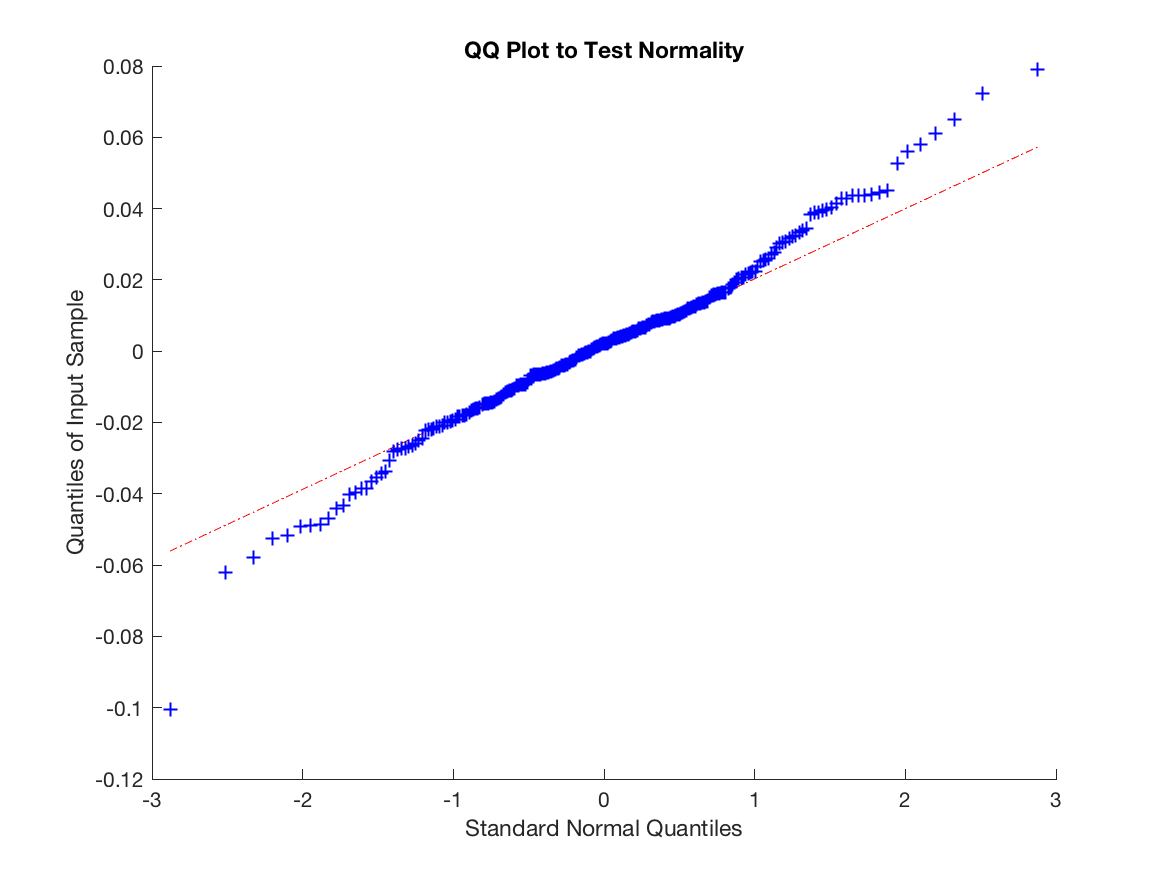
\includegraphics[width=0.8\linewidth]{qqplot}
		\caption{Determining Brownian Fit}
		\label{fig:test1}
	\end{minipage}%
	\begin{minipage}{.5\textwidth}
		\centering
		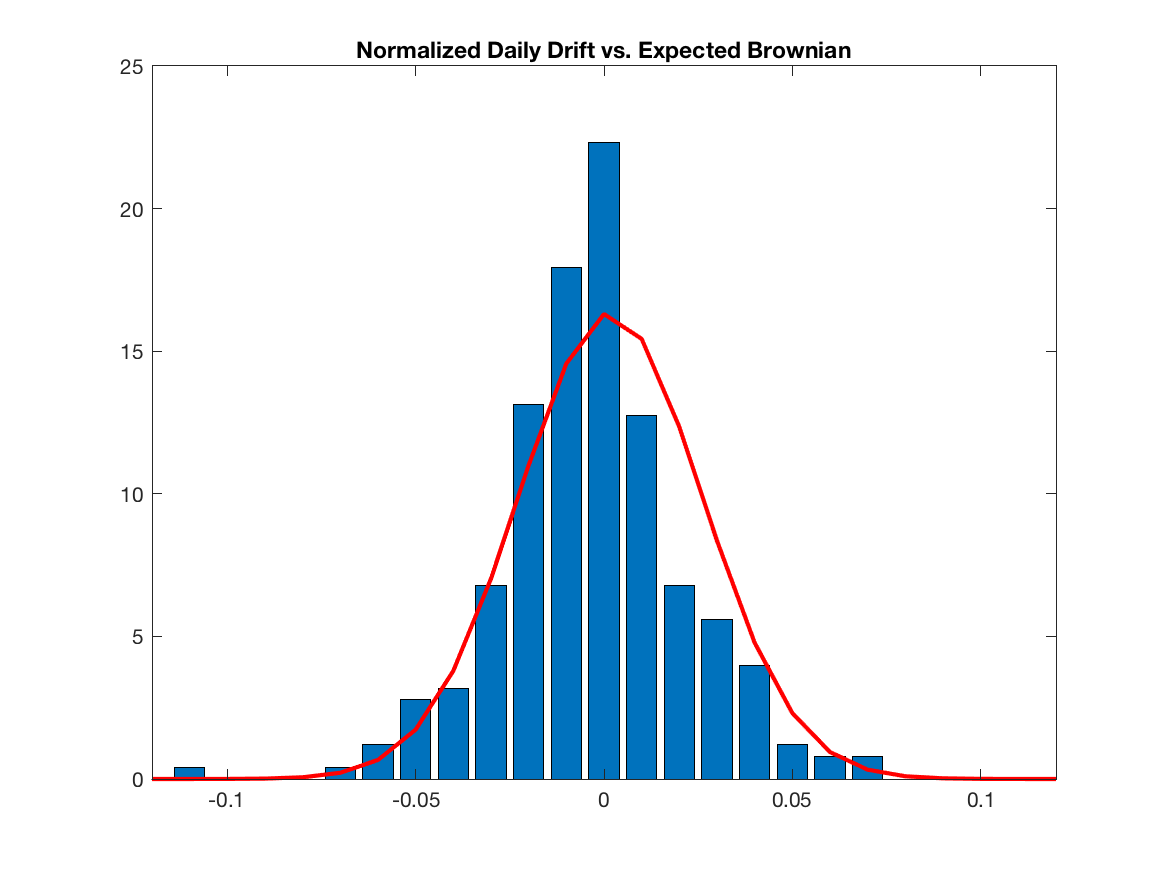
\includegraphics[width=0.8\linewidth]{brownianHist}
		\caption{Normalized Distribution}
		\label{fig:test2}
	\end{minipage}
\end{figure}
 

\section{Expected return}
Expected return is the log ratio of the return from investing today (t=0) and some future time t minus the market rate. This will determine the premium return. 

\begin{align}
E(return) =& log(\frac{X(t)e^{-\alpha t}}{X(0)})\\
=& (\mu + \sigma^2/2 - \alpha)t\\
=& (0.6275+ 0.2174/2 - 0.375)t\\
=& 0.6987 \qquad \square
\end{align}

The likelihood of seeing a 5\% return next year would require an actual rate of return of 8.75\%. Given the fact that we can approximate this using Brownian motion, the probability of the return being greater than 8.75\% can be written as:

\begin{align}
P\{return > .0875\} =& 1-\Phi(\frac{.0875 - 0.6275}{\sqrt{ 0.2174}})\\
=& 1-\Phi(-1.15814)\\
=& 87.66\%
\end{align}

\section{Risk neutral measure}
Risk, or beta, is essentially a measure of volatility of the stock above market rate. It can be equated as:
$$\alpha - \sigma^2/2 = .0375 - 0.2174/2 = -0.0712$$

The volatility of the stock remains 0.2174.

\section{Expected return for risk neutral measure}
Given that the expectation of risk-neutral return, $\mu$, is negative, I would choose not to invest, therefore, my return would be \$0. I would instead invest in the market and see a return of $\alpha$, 3.75\%.

\section{Derive Black-Scholes formula}

\begin{align}
\mathbb{E}_q[e^{-\alpha t }[X(t)-K]^+-c]=&0\\
c =& e^{-\alpha t } \mathbb{E}_q[X(t)-K]^+\\
=& e^{-\alpha t } \mathbb{E}_q[X_0e^{Y(t)}-K]^+\\
=& e^{-\alpha t } \frac{1}{\sqrt{2\pi t \sigma^2}}\int_{-\infty}^{\infty} (X_0e^{Y(t)}-K)^+e^{\frac{-(y-(\mu t)^2)}{2t\sigma^2}}\\
=& e^{-\alpha t } \frac{1}{\sqrt{2\pi t \sigma^2}}\int_{log(K/X_0)}^{\infty} (X_0e^{Y(t)}-K)^+e^{\frac{-(y-(\mu t)^2)}{2t\sigma^2}}\\
\text{Given the following change of variabeles:}&\\
\text{let } z =  (y - \mu t)/\sqrt{t\sigma^2}&\\
y = \sqrt{t\sigma^2}z + \mu t&\\
dy = \sqrt{t\sigma^2}dz&\\
\text{int limit: } a = \frac{log(K/X_0)-\mu t}{\sqrt{t\sigma^2}}&\\
=& e^{-\alpha t } \frac{1}{\sqrt{2\pi}}\int_{a}^{\infty} (X_0e^{\sqrt{t\sigma^2}z + \mu t}-K)^+e^{\frac{z^2}{2}}dz\\
let \quad l1 =& \frac{1}{\sqrt{2\pi}}\int_{a}^{\infty} (X_0e^{\sqrt{t\sigma^2}z + \mu t})e^{\frac{z^2}{2}}dz\\
=& \frac{X_0e^{\mu t+t\sigma^2/2}}{\sqrt{2\pi}}\int_{a}^{\infty} e^{-(z-\sqrt{t\sigma^2})/2)}dz\\
\text{Given a change of variables: }=& \\
let \qquad u = z-\sqrt{t\sigma^2}&\\
du = dz&\\
\text{int limit: } b = \frac{log(K/X_0)-\mu t}{\sqrt{t\sigma^2}} - \sqrt{t\sigma^2}&\\
=& \frac{X_0e^{\mu t+t\sigma^2/2}}{\sqrt{2\pi}}\int_{b}^{\infty} e^{-u/2}du\\
=&X_0e^{\mu t+t\sigma^2/2}Q(b)\\
let \quad l2 =&\frac{K}{\sqrt{2\pi}}\int_{a}^{\infty}e^{\frac{z^2}{2}}dz = KQ(a)\\
c =& e^{-\alpha t }(l1-l2) = e^{-\alpha t }(X_0e^{\mu t+t\sigma^2/2}Q(b) - KQ(a))\\
c=& X_0Q(a - \sqrt{t \sigma^2}) - e^{-\alpha t }KQ(a) \qquad \square
\end{align}

\section{Determine option price}

Using the following code, I determined c to be 0.7190, 0.2941, and 0.1243 for K =0.8, 1, 1.2 respectively.

\begin{lstlisting}
alph = .0375;

X0 = close_price(1);
Ex = X0*exp(mu+var/2);
K = [0.8 1 1.2]*Ex;
c = zeros(1, length(K));
risk_nuetral = alph - var/2;

for k=K
a = (log(k/X0)-risk_nuetral)/sqrt(var);
b = a - sqrt(var);
QA = 1-normcdf(a, 0, 1);
QB = 1 - normcdf(b, 0, 1);

c(K==k) = X0*QB-exp(-alph)*k*QA;
end

disp(option_price);
\end{lstlisting}

\end{document}
